\vspace{-0.5em}
\section{Motivating Examples}
\label{sec:motivating-examples}
\vspace{-0.5em}

We look at the namespaces of 3 applications.  Each is from different domains
and this list is not meant to be exhaustive.  To highlight the scalability
challenges for file system metadata management, we focus on large scale systems
in high performance computing, high energy physics, and large scale
simulations. Large lists represent common problems in each of these domains.
To make our results reproducible, this paper adheres to The Popper
Convention~\cite{jimenez:ipdpsw17-popper} so experiments can be examined in
more detail, or even re-run, by visiting the \texttt{[source]} link next to
each figure. 

% This discussion is irrelevant since we are focusing on namespace size/overhead
%We benchmark over Ceph (Jewel version) with \(n\) object storage daemons
%(OSDs), 1 metadata server (MDS), 1 monitor server (MON), and 1 client.  We use
%3 OSDs because it sustains 16 concurrent writes of 4MB at 600MB/s for 2
%minutes. 250MB/s is the max speed of the SSDs, so the setup achieves 80\% of
%the cluster SSD bandwidth.  We use CephFS, the POSIX-compliant file system that
%uses Ceph's RADOS object store~\cite{weil:osdi2006-ceph}, as the underlying
%file system.  This analysis focuses on the file system metadata RPCs between
%the client and metadata server and does not include the RPCs needed to write
%and read actual data.  CephFS uses a cluster of metadata servers to service
%file system metadata requests~\cite{weil:sc2004-dyn-metadata} and to
%characterize the workload, we instrumented the metadata server to track the
%number of each request type\footnote{This code was merged into the Ceph
%project.}.
\begin{figure*}[tb]
    \centering
    \begin{subfigure}[b]{.45\linewidth}
      \centering
      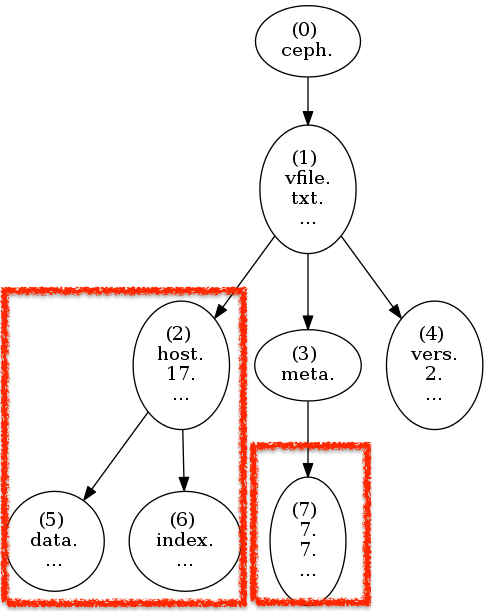
\includegraphics[width=1\linewidth]{figures/tree_plfs.png} 
      \caption{PLFS file system tree}\label{fig:tree_plfs}
   \end{subfigure}
   \begin{subfigure}[b]{.45\linewidth}
     \centering
     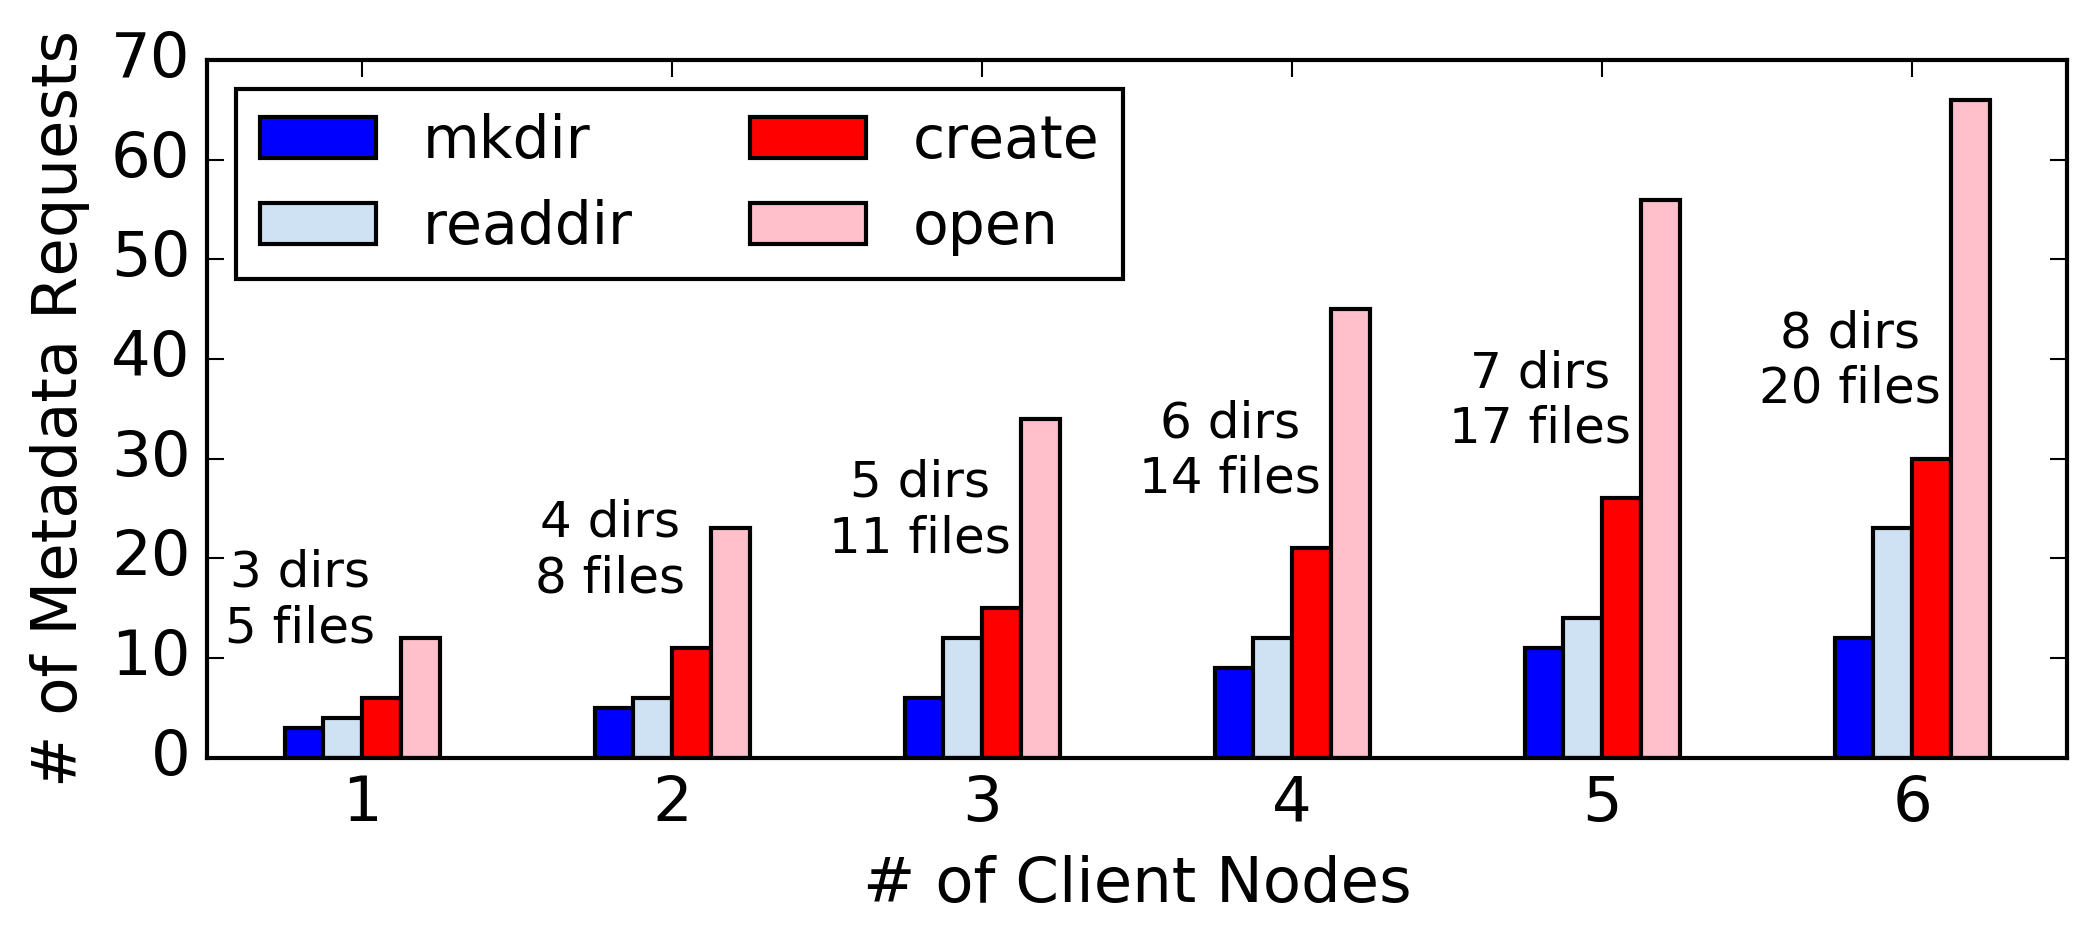
\includegraphics[width=1\linewidth]{figures/plfs_problem.png} 
     \caption{[\href{https://github.com/michaelsevilla/tintenfisch-popper/blob/master/experiments/n1/vizualize.ipynb}{source}]
     PLFS metadata size and operations.}
     \label{fig:plfs_problem}
   \end{subfigure}
\caption{PLFS file system metadata. (a) shows that the namespace is structured
and predictable; the pattern (solid line) is repeated for each hosts. In this
case, there are three hosts so the pattern is repeated two more times. (b)
shows that the namespace scales linearly with the number of clients.  This
makes reading and writing difficult using RPCs so decoupled namespace must be
used to reduce the number of RPCs.}
\end{figure*}


\vspace{-0.5em}
\subsection{High Performance Computing: PLFS}
\label{sec:plfs}
\vspace{-0.5em}

% What is the problem the authors are trying to solve?
Checkpointing performs small writes to a single shared file but because file
systems are optimized for large writes, performance is poor.
PLFS~\cite{bent_plfs_2009} solved the checkpoint-restart problem by mapping
logical files to physical files on the underlying file system. The solution
targets N-1 strided checkpoints, where many processes write small IOs to
offsets in the same logical file.  Each process sequentially writes to its own,
unshared data file in the hierarchical file system and records an offset and
length in an index file. Reads aggregate index files into a global index file,
which it uses as a lookup table for identifying offsets into the logical file. 

%It easier for
%applications to write checkpoints to a single file with unaligned writes of
%varying length (N-1) but general-purpose distributed file systems are designed
%for writes to different files (N-N).  The general problem is that the
%application understands the workload but cannot communicate a solution to the
%storage system. The common solution is for the file system to expose
%configurations that describe alignment requirements but this forces application
%developers to specify ``magic numbers" for parameters like write
%size~\cite{bent_plfs_2009} or stripe size~\cite{behzad:sc2013-autotuning},
%which are hard to find and may not even exist.  Another solution is to add
%middleware ({\it i.e.} software that sits between the application and the
%storage system) to translate the data into a format the storage system performs
%well at. 

%% What is the problem?
%The problem is that the underyling file system cannot keep up with the metadata
%load imposed by PLFS. PLFS creates an index entry for every write, which
%results in large per-processes tables~\cite{grider:pc17-diddlings}. This makes
%reading or scanning a logical file slow because PLFS must construct a global
%index by reading each process's local index. This process incurs a
%\texttt{readdir} and, if the file is open by another process, an additional
%\texttt{stat()} because metadata cannot be cached in the
%container~\cite{bent_plfs_2009}.

%\subsubsection{System Architecture}
%@noah: there is an index because applications do not have regular IO

% What is the authors' approach or solution?
%PLFS maps an application's preferred data layout into one that the file system
%performs well on. 

% How does PLFS create namespaces
\textbf{Namespace Description}: when PLFS maps a single logical file to many
physical files, it deterministically creates the namespace in the backend file
system.  For metadata writes, the number of directories is dependent on the
number of clients nodes and the number of files is a function of the number of
client processes.  A directory called a container is created per node and
processes write data and index files to the container assigned to their host.
So for a write workload ({\it i.e.} a checkpoint) the underlying file system
creates a deep and wide directory hierarchy, as shown in
Figure~\ref{fig:tree_plfs}.  The \texttt{host*} directory and
\texttt{data*}/\texttt{index} files (denoted by the solid red line) are created
for every node in the system. The pattern is repeated twice (denoted by the
dashed blue line) in the Figure, representing 2 additional hosts each with 1
process.

\textbf{Namespace Size}: Figure~\ref{fig:plfs_problem} scales the number of
clients and plots the total number of files/directories (text annotations) and
the number of metadata operations needed to write and read a PLFS file.  The
number of files is \(2\times(\text{\# of processes})\).  So for 1 million
processes each checkpointing a portion of a 3D simulation, the size of the
namespace will be 2 million files.  RPC-based approaches like
IndexFS~\cite{ren:sc2014-indexfs} have been shown to struggle with metadata
loads of this size but decoupled namespace approaches like
DeltaFS~\cite{zheng:pdsw2015-deltafs} report up to 19.69 million creates per
second, so writing checkpoints is largely a solved problem.

% How does PLFS read the namespace
For reading a checkpoint, clients must coalesce index files to reconstruct the
PLFS file. Figure~\ref{fig:plfs_problem} shows that the read metadata requests
(``readdir" and ``open") outnumber the create requests by a factor of
\(4\times\). Metadata read requests are notoriously
slow~\cite{carns:ipdps09-pvfs, eshel:fast10-panache}, so like create requests,
RPCs are probably untenable. If the checkpoint had been written with the
decoupled namespace approach, file system metadata would be scattered across
clients so metadata would need to be coalesced before restarting the
checkpoint. If the metadata had already been coalesced at some point they would
still need to be transferred to the client. Regardless, both decoupled
namespace scenarios require moving and materializing the file system namespace.
Current efforts improve read scalability by reducing the space overhead of the
index files themselves~\cite{he:hpdc13-plfs-patterns} and transferring index
files after each write~\cite{grider:pc17-diddlings} but these approaches target
the transfer and materialization of the index file data, not the index file
metadata.

\textbf{Takeaway}: the PLFS namespace scales with the number of client
processes so RPCs are not an option for reading or writing.  Decoupling the
namespace helps writes but then the read performance is limited by the speed of
transferring file system metadata across the network to the reading client {\it
in addition} to reading the contents of the index files themselves.

\vspace{-0.5em}
\subsection{High Energy Physics: ROOT}
\label{sec:hep}
\vspace{-0.5em}

% the data
The High Energy Physics (HEP) community uses a framework called ROOT to
manipulate, manage, and visualize data about proton-proton collisions collected
at the large hadron collider (LHC). The data is used to re-simulate phenomena
of interest for analysis and there are different types of reconstructions each
with various granularities. The data is organized as nested, object oriented
event data of arbitrary type ({\it e.g.}, particle objects, records of
low-level detector hit properties, etc.).  Physicists analyze the data set by
downloading interesting events, which are stored as a list of objects in ROOT
files.  ROOT file data is accessed by consulting metadata in the header and
seeking to a location in the bytestream, as shown in
Figure~\ref{fig:tree_hep_a}.  The ROOT file has both data and ROOT-specific
metadata called Logical Record Headers (LRH).  For this discussion, the
following objects are of interest: a ``Tree" is a table of a collection of
events, listed sequentially and stored in a flat namespace; a ``Branch" is a
data container representing columns of a Tree; and ``Baskets" are byte ranges
partitioned by events and indexed by LRHs.  Clients request Branches and data
is transferred as Baskets; so Branches are the logical view of the data for
users and Baskets are the compression, parallelization, and transfer unit.  The
advantages of the ROOT framework is the ability to (1) read only parts of the
data and (2) easily ingest remote data over the network.  

%Reconstruction takes detector conditions ({\it
%e.g.}, alignment, position of the beam, etc.) as input.  
%Data is streamed from
%the LHC into large immutable datasets, stored publicly in data centers around
%the world.  

% ROOT files
%In summary, ROOT files are self-describing files containing data located with
%metadata and serialized/de-serialized with the ROOT framework.  
%Much of the
%development was done at CERN in parallel with other HPC ventures. As a result,
%the strategies are similar to techniques used in HDF5, Parquet, and Avro.

% WHat does ROOT have?
%\begin{itemize}
%
%  \item subdirectories within a file, for organization like HDF5
%
%  \item serialization of any type of C++ object, like Python's pickle, but for
%  C++
%
%  \item embedded schema with schema evolution like Avro
%
%  \item columnar storage of large sets of events, like the Dremel/Parquet
%  shredding algorithm (called "splitting" in ROOT)
%
%  \item selective reading, also like Dremel/Parquet (the "prune" feature of
%  SparkSQL DataFrames)
%
%  \item mutable content; a ROOT file is effectively a single-user object
%  database (but without ORM: the data are fundamentally not relational— maybe
%  "document store" would be a better word for what it's doing). Not all
%  operations are guaranteed to be atomic or thread-safe (hence "single-user").
%
%\end{itemize}
%
%Optimizations and trade-offs are controlled with configurations. For example,
%the \texttt{splitlevel} parameter controls the data layout, {\it i.e.} whether
%it is organized more closely to rowwise or columnar.  Low values store columns
%values as tuples in entries ({\it i.e.} \texttt{splitlevel=0} stores all column
%values as tuples in each entry) while high values make the data more
%columnar-based. Other parameters control the size and shape of hierarchical
%structure of the ROOT file include events per file, target Basket size, cluster
%size, compression algorithm and level, and alignment of objects with disk
%pages.


\begin{figure*}[tb]
    \centering
    \begin{subfigure}[b]{.25\linewidth}
      \centering
      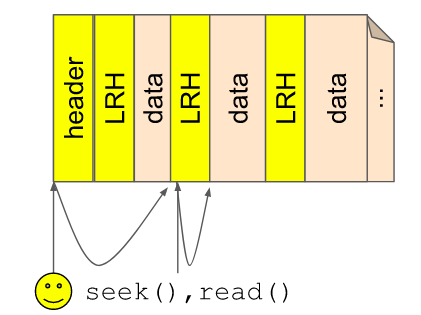
\includegraphics[width=1.0\linewidth]{figures/tree_hep_a.png} 
      \caption{file approach}
      \label{fig:tree_hep_a}
    \end{subfigure}
    \begin{subfigure}[b]{.25\linewidth}
      \centering
      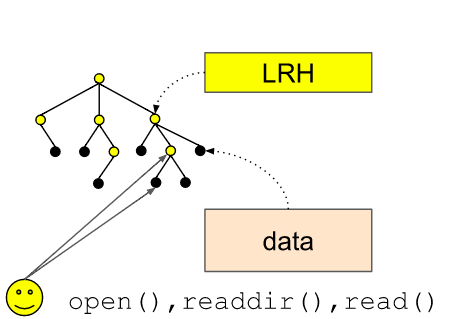
\includegraphics[width=1.0\linewidth]{figures/tree_hep_b.png} 
      \caption{namespace approach}
      \label{fig:tree_hep_b}
    \end{subfigure}
    \begin{subfigure}[b]{.4\linewidth}
      \centering
      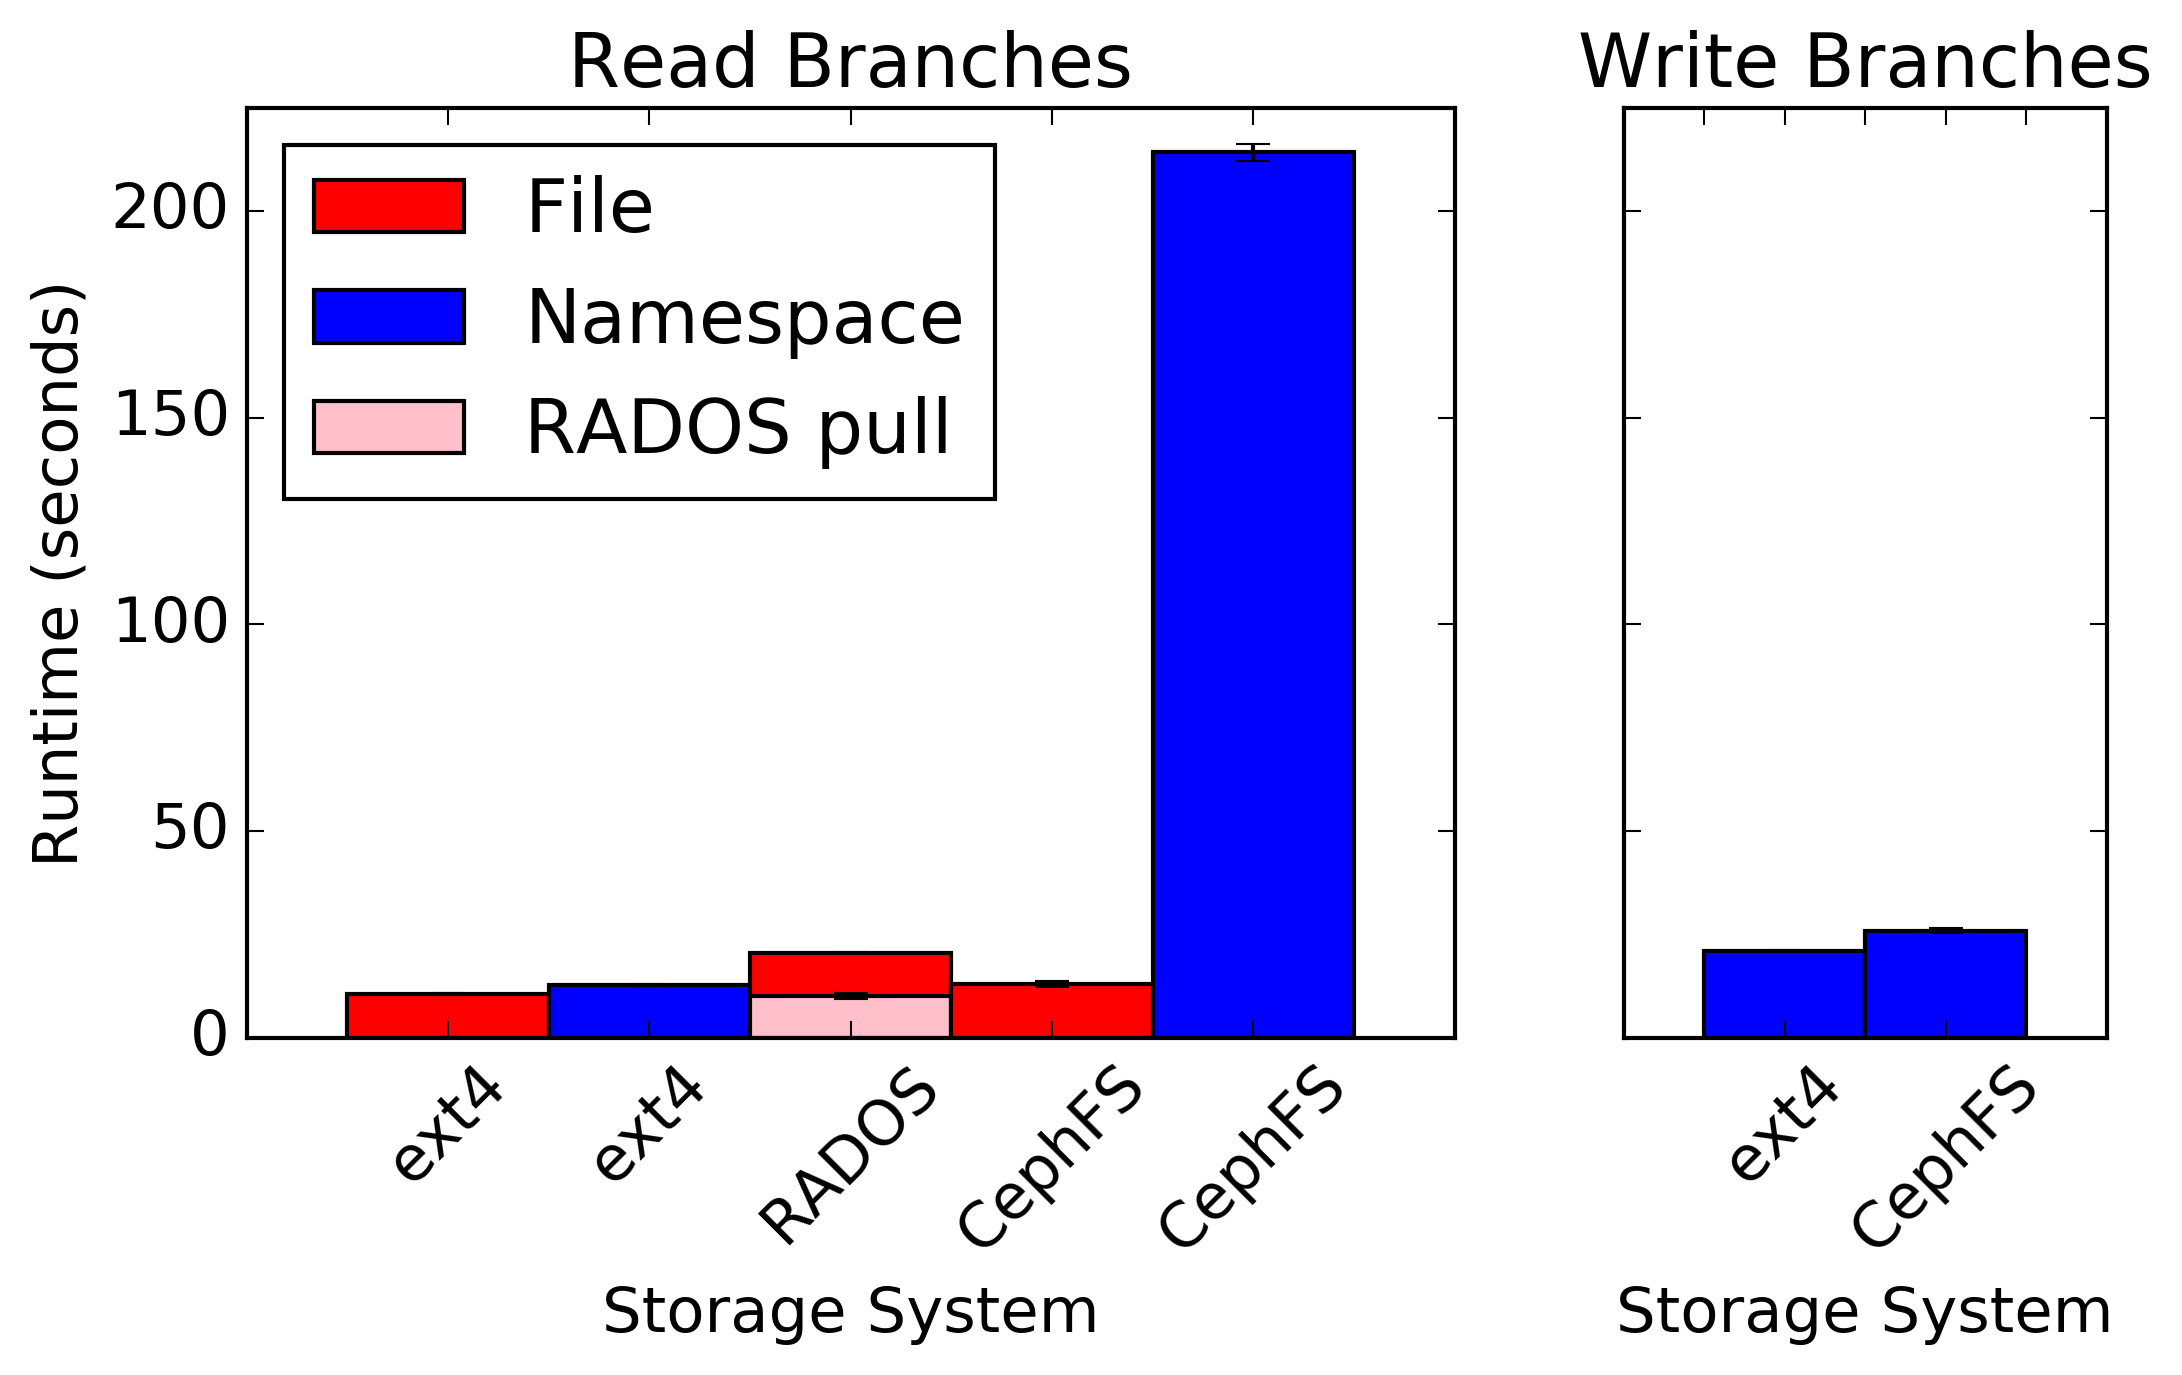
\includegraphics[width=1\linewidth]{figures/hep_runtime.png}
      \caption{
      [\href{https://github.com/michaelsevilla/tintenfisch-popper/blob/master/pipelines/hep/visualize/viz.ipynb}{source}]
      ROOT metadata size and operations}
      \label{fig:hep_runtime}
    \end{subfigure}
\caption{ROOT file system metadata. (a) file approach: stores data in a single
ROOT file, where clients read the header and seek to data or metadata (LRH); a
ROOT file stored in a distributed file system will have IO read amplification
because the striping strategies are not aligned to Baskets. (b) namespace
approach: stores Baskets as files so clients read only data they need. In (c),
``Namespace" is the runtime of reading a file per Basket and ``File" is the
runtime of reading a single ROOT file. RPCs are slower because of the metadata
load and the overhead of pulling many objects.  Decoupling the namespace uses
less network (because only metadata and relevant Baskets get transferred) but
incurs a metadata materialization overhead.}
\end{figure*}

\textbf{Namespace Description}: the HEP community is running into scalability
problems.  The current effort is to integrate the ROOT framework with Ceph. But
naive approaches such as storing ROOT files as objects in an object store or
files in a file system have IO read amplification ({\it i.e.} read more than is
necessary); storing as an object would pull the entire GB-sized blob and
storing as a file would pull more data than necessary because the file stripe
size is not aligned to Baskets.  To reduce IO read amplification the namespace
approach~\cite{pivarski:indico17-root} views a ROOT file as a namespace of
data.  Physicists ask for Branches, where each Branch can be made up of
multiple sub-Branches ({\it i.e.} \texttt{Events/Branch0/Branch1}), similar to
pathname components in a POSIX IO file name. The namespace approach
partitions the ROOT file onto a file system namespace, as shown in
Figure~\ref{fig:tree_hep_b}. File system directories hold Branch metadata,
files contain Baskets, and clients only pull Baskets they care about.

%At the top of the namespace are Keys, each containing pointers to groups of
%Branches. For example, ``MetaData" has data about the run and ``Events" has
%all the proton-proton activity.  is not enough metadata to reconstruct which
%Branches belong to which events.  tely, current file system do not have this
%many inodes and this setup would require extra metadata to combine TBranches
%into objects.

%%\begin{figure}[t]
%%  \centering
%%  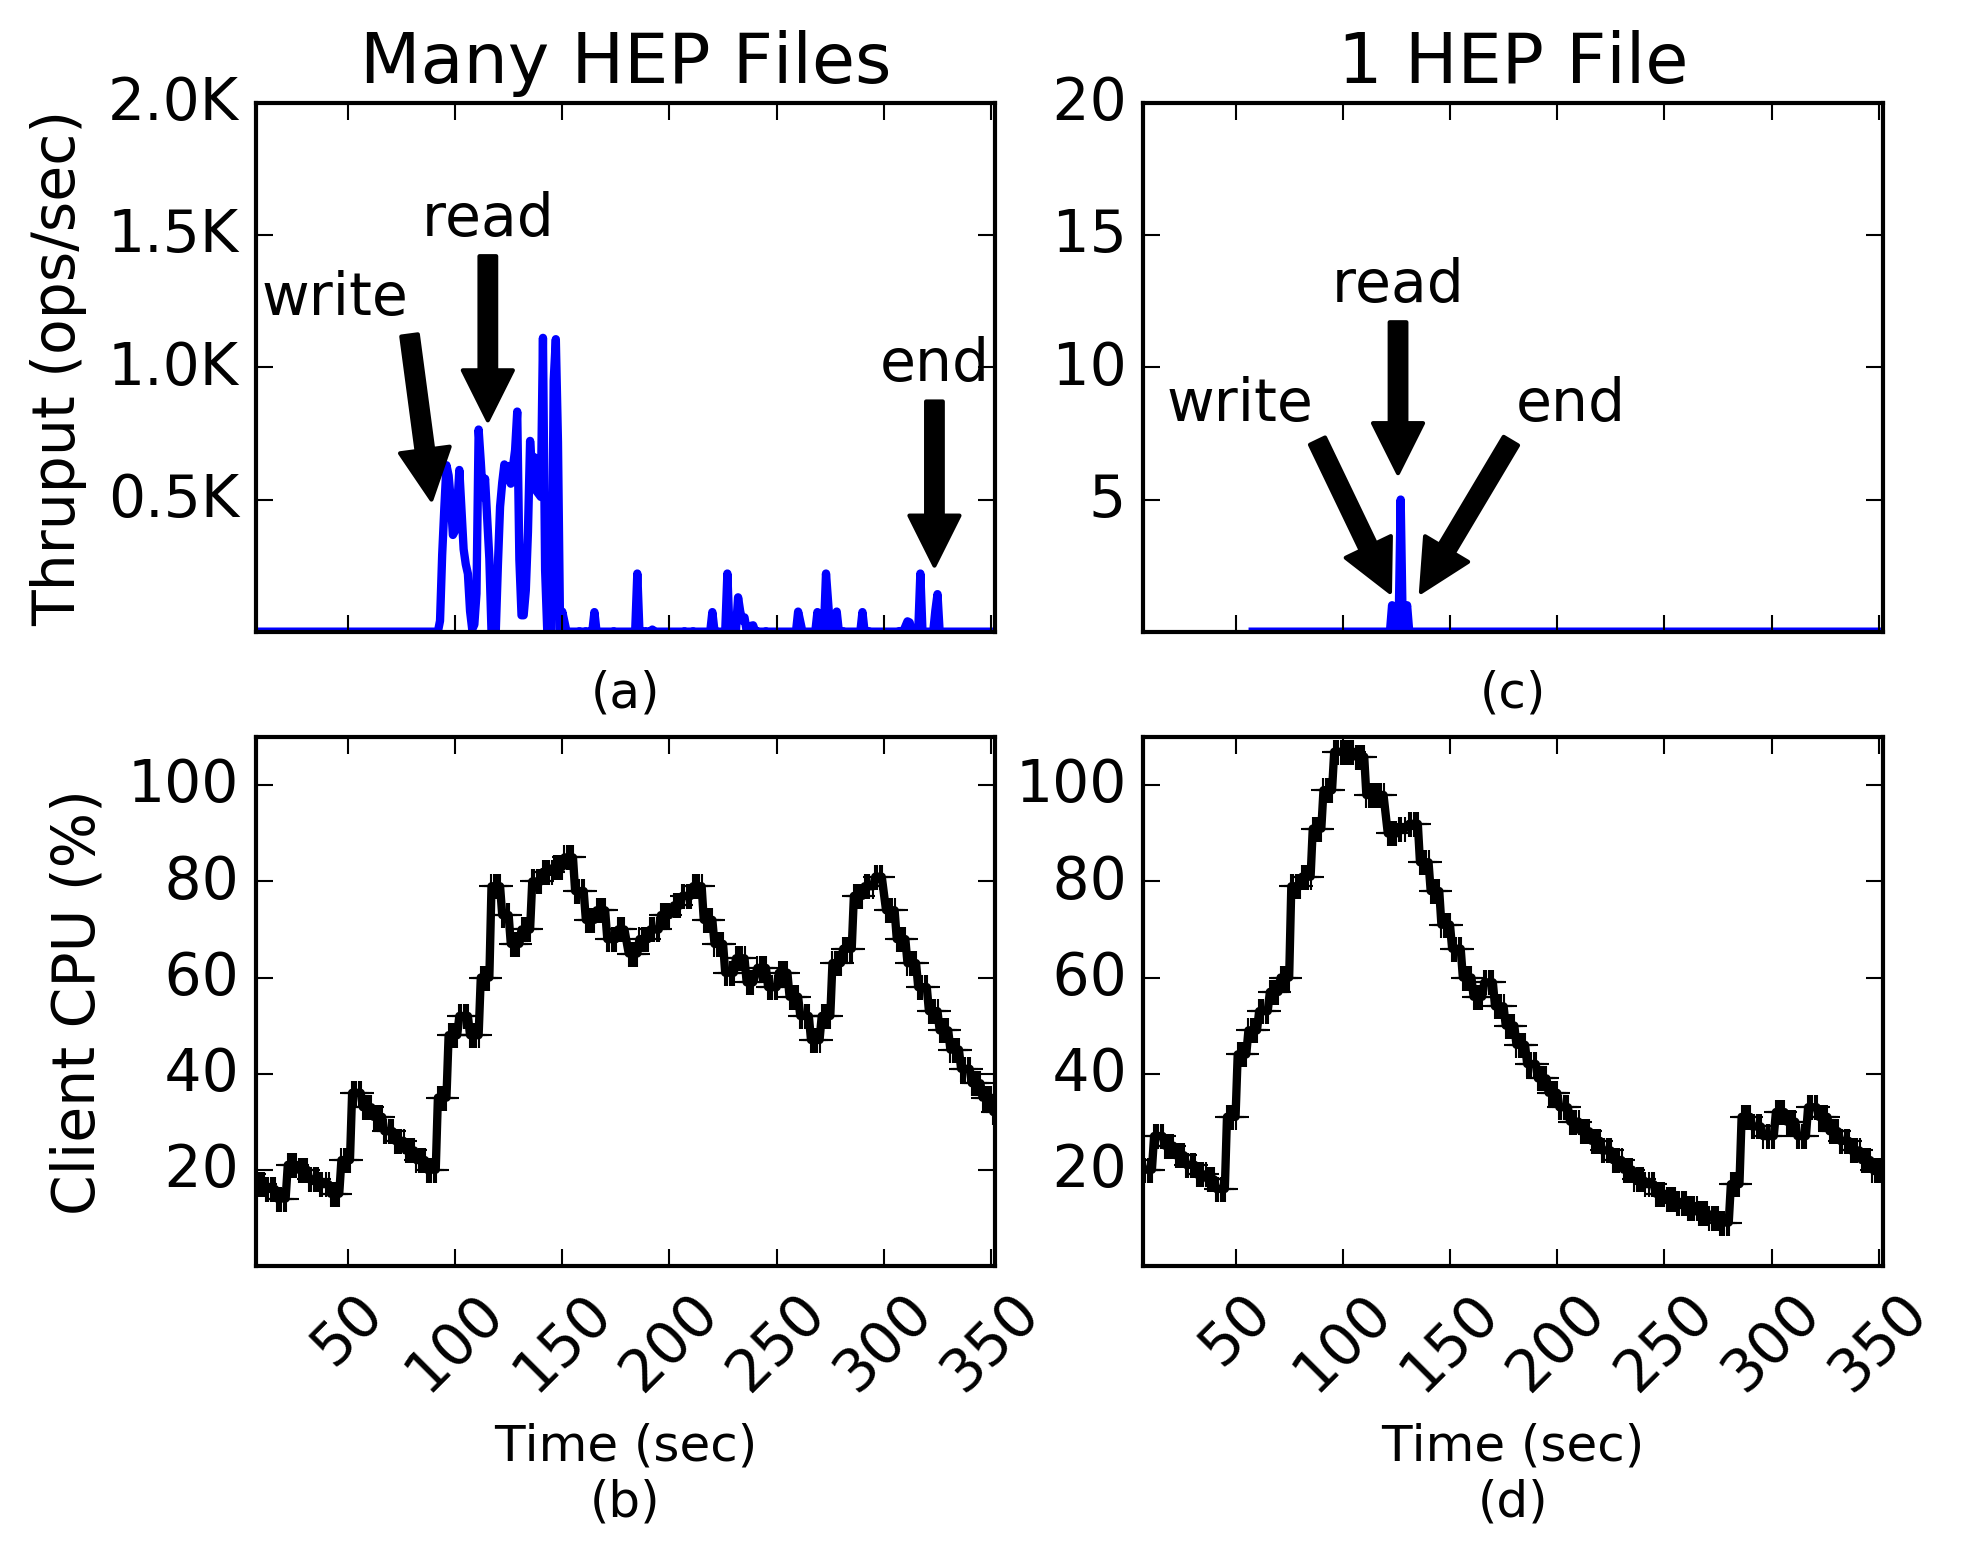
\includegraphics[width=90mm]{figures/hep_problem.png}
%%  \caption{Reading and writing high-energy physics (HEP) data as many files
%%allows physicists to read just the data they care about. But using this
%%namespace approach sends many RPCs to the metadata server (a), resulting in
%%worse performance and lower CPU utilization at the client (b). Alternatively,
%%using the traditional file approach has IO amplification because all data moves
%%over the network but less RPCs (c), better performance, and higher client CPU
%%utilization (d).}
%%  \label{fig:hep_problem}
%%\end{figure}

%We benchmark the write and read overhead of storing HEP data with the file
%approach stored as one object in an object store, with the file approach stored
%as one file in a file system, and with the namespace approach stored as many
%files in a file system.  The file approaches are deployed without any changes
%to the ROOT framework. For the namespace approach, HEP-specific metadata is
%mapped onto the file system namespace. In CephFS, Baskets are stored in Ceph
%objects and the Branch hierarchy is managed by the metadata server.  Clients
%contact the metadata server with a Branch request, receive back the Branch
%hierarchy necessary to name the Ceph object containing the Basket as well as
%the deserialization metadata necessary to read the object.  The workload is a
%list of Branch accesses from a trace of the NPTupleMaker high energy physics
%application. Each Branch access is:
%
%\texttt{Branch0/Branch1,3,1740718587,5847,97,136}
%
%where the tuple is the full Branch name, Basket number, offset into the ROOT
%file, size of the Basket, start entry of the Basket, and end entry of the
%Basket.  For the file approach, we use the offset into the ROOT file and the
%size of the Basket.  In setup 1, the ROOT file is pulled locally and the
%Branches are read from the file. In setup 2, the offset and size of the read
%are sent to the CephFS metadata server.  For setup 3, the full Branch name and
%Basket number are used to traverse the file system namespace.

%The start and end entry of the Basket are the logical records that
%bookend the Basket ({\it e.g.}, for a start entry of 10 and end entry of 20 for
%a Basket storing user ages, the start entry is user 10's age and the end entry
%is user 20's age).  

\textbf{Namespace Size}: storing this metadata in a file system would overwhelm
most file systems in two ways: (1) too many inodes and (2) per-file overhead.
To quantify (1), consider the Analysis Object Dataset which has a petabyte of
data sets made up of a million ROOT files each containing thousands of
Branches, corresponding to a billion files in the namespace approach.  To
quantify (2), the read and write runtime over six runs of replaying a trace of
Branch access from the NTupleMaker application is shown in
Figure~\ref{fig:hep_runtime}, where the \(x\)-axis is approaches for storing
ROOT data.  Using the namespace approach with RPCs is far slower because of the
metadata load and because many small objects are pulled over the network.
Although the file approach reads more data than is necessary since the stripe
size of the file is not aligned to Baskets, the runtime is still \(16.6\times\)
faster. Decoupling the namespace is much faster for the namespace approach but
the cost of materializing file system metadata makes it slower than the file
approach.  Note that this is one (perhaps pessimistic) example workload; the
ROOT file is 1.7GB and 65\% of the file is accessed so the namespace approach
might be more scalable for workloads that access fewer Baskets.

%The reason is shown in Figure~\ref{fig:hep_problem}. The file system metadata
%accesses, characterized by many \texttt{open()} requests, incur many RPCs.
%This causes worse performance and lower client CPU utilization compared to
%reading a single ROOT file.  So the cost of read amplification in the file
%approach is offset by the cost of doing namespace operations. 

\textbf{Takeaway}: the ROOT namespace stores billions of files and we show that
RPCs overwhelm a centralized metadata server. Decoupling the namespace helps
writes but then the read performance is limited by (1) the speed of
transferring file system metadata across the network and (2) the cost of
materializing parts of the namespace that are not relevant to the workload.

\vspace{-0.5em}
\subsection{Large Scale Simulations: SIRIUS}
\vspace{-0.5em}

SIRIUS~\cite{klasky:journal16-sirius} is the Exascale storage system being
designed for the Storage System and I/O (SSIO)
initiative~\cite{ross:report14-ssio}. The core tenant of the project is
application hints that allow the storage to reconfigure itself for higher
performance using techniques like tiering, management policies, data layout,
quality of service, and load balancing.  SIRIUS uses a metadata service called
EMPRESS~\cite{lawson:pdsw17-empress}, which is an SQLite instance
that stores user-defined metadata for bounding boxes ({\it i.e.} a
3-dimensional coordinate space).  EMPRESS is designed to be used at any
granularity, which is important for a simulation space represented as a 3D
mesh. By granularity, we mean that metadata access can be optimized per
variable ({\it e.g.}, temperature, pressure, etc.), per timestamp, per run, or
even per set of runs (which may require multiple queries).  EMPRESS is also
designed to scale-out via additional independent instances, where one client
per node queries the entire space of interest by contacting EMPRESS servers,
coalesces results, and distributes them using MPI messages.

%So clients reading from SIRIUS will first
%contact EMPRESS with the queries for all data, all of 1 variable, all of a few
%variables, a plane in each dimension, an arbitrary rectangular subset, or an
%arbitrary area on an orthogonal plane, and EMPRESS will return a list of
%objects. Armed with this list, the client contacts the object storage system
%(in our case this is RADOS, Ceph's object store) and reads relevant data.

\begin{figure}[tb]
\centering
  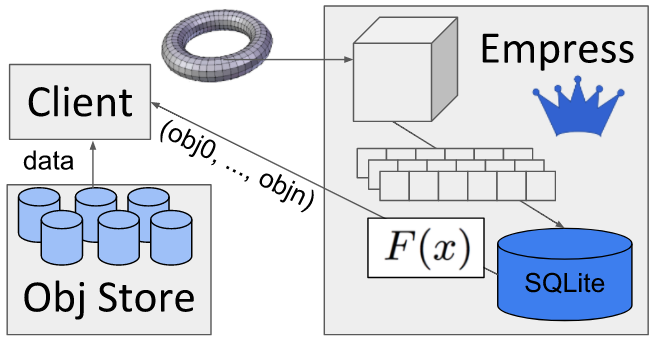
\includegraphics[width=0.8\linewidth]{figures/empress.png}
  \caption{SIRIUS uses EMPRESS to store metadata for bounding boxes in a 3D
torus. Coordinates and user-defined metadata are stored in SQLite and object
names are calculated using a partitioning function (\(F(x)\)). One approach is to
return a list of object names to the client}
  \label{fig:empress}
\end{figure}

\textbf{Namespace Description}: the database has columns for the application
ID, run ID, timestamp, variable name, feature name, and bounding box
coordinates.  The global space is partitioned into non-overlapping, regular
shaped cells.  Each row in the database is duplicated for each variable in the
simulation because variables may have a different partitioning of the global
space; for example temperature is computed for every cell while pressure is
computed for every \(n\) cells.  Figure~\ref{fig:empress} only has three
variables, represented by the rows of boxes but most simulations will have a
minimum of 10 variables.

\textbf{Namespace Size}: a back-of-the-envelope calculation for the number of
object names for a single run is:
\vspace{-0.5em}
\[\frac
  {(\text{processes})\times
   (\text{data/process})\times
   (\text{variables})\times
   (\text{timesteps})}
  {(\text{object size})}
\]
\vspace{-0.5em}
%\[=\frac
%  {(1*10^6)\times
%   (8*10^{9})\times
%   (10)\times
%   (100)}
%   {(8*10^6)}
%  = 1*10^{12}
%\text{ objects} \]

We calculate \(1*10^{12}\) (1 trillion) objects for a simulation space of
\(1\text{K}\times1\text{K}\times1\text{K}\) cells containing 8 byte floats.  We
use 1 million processes, each writing 8GB of data for 10 variables over 100
timesteps and an object size of 8MB (the optimal object size of Ceph's object
store).  The data per process and number of variables are scaled to be about
1/10 of each processes local storage space, so about 80GB. 100 timesteps is
close to 1 timestep every 15 minutes for 24 hours. 

As we integrate EMPRESS with a scalable object store, mapping bounding box
queries to object names for data sets of this size is a problem. Clients query
EMPRESS with bounding box coordinates\footnote{Users usually track bounding
boxes of interest by tagging features at write time.} and EMPRESS must provide
the client with a list of (possibly overlapping) object names.  These lists can
be very large when applications query multiple runs each containing trillions
of objects.  One option is to calculate object names at write time and store
them with bounding box coordinates but this would result in a large storage
footprint and long transfer times for sending the object name list to the
client.  Another option is shown in Figure~\ref{fig:empress}; coordinates for
variables (rows of gray boxes) are stored in the database and object name lists
are calculated using the \(F(x)\) partitioning function at read time and sent
back to the client. This solves the storage footprint problem but not the long
transfer times.  Even after receiving the object name list, the client may need
to do more filtering for object names at the ``edge" of the feature of
interest.

%For distributed EMPRESS, the storage footprint may not be as much
%of an issue but the trade-off is transferring parts of the object name list
%over the network as reads must be centralized at the designated read process on
%each client. 
%Listing large numbers of items in file systems is notoriously slow and studies
%on \texttt{ls} have shown the operation to be especially
%heavy-weight~\cite{carns:ipdps09-pvfs, eshel:fast10-panache}.  

\textbf{Takeaway}: SIRIUS stores trillions of objects for a single large scale
simulation run and applications often access multiple runs. These types of
queries return a large list of object names so the bottleneck is managing,
transferring, and traversing these lists. The size of RPCs is the problem, not
the number. POSIX IO hierarchical namespaces may be a good model for
applications to access simulation data but another technique for handling the
sheer size of these object name lists is needed.

% solution: compact the metadataa required to name objects and generate only
% what you need
